\documentclass[14pt, a4paper]{report}
\usepackage[utf8]{inputenc}
\usepackage[english, russian]{babel}

\usepackage{graphicx}
\usepackage{listings}
\usepackage{color}

\usepackage{amsmath}
\usepackage{pgfplots}
\usepackage{url}
\usepackage{flowchart}
\usepackage{tikz}
\DeclareGraphicsExtensions{.pdf,.png,.jpg,.svg}
\usetikzlibrary{shapes, arrows}

\usepackage{pgfplotstable}

\renewcommand\contentsname{Содержание}

\usepackage{geometry}
\geometry{left=3cm}
\geometry{right=1cm}
\geometry{top=2cm}
\geometry{bottom=2cm}

% Для листинга кода:
\lstset{ %
language=python,                 % выбор языка для подсветки (здесь это С)
basicstyle=\small\sffamily, % размер и начертание шрифта для подсветки кода
numbers=left,               % где поставить нумерацию строк (слева\справа)
numberstyle=\tiny,           % размер шрифта для номеров строк
stepnumber=1,                   % размер шага между двумя номерами строк
numbersep=-5pt,                % как далеко отстоят номера строк от подсвечиваемого кода
showspaces=false,            % показывать или нет пробелы специальными отступами
showstringspaces=false,      % показывать или нет пробелы в строках
showtabs=false,             % показывать или нет табуляцию в строках
frame=single,              % рисовать рамку вокруг кода
tabsize=2,                 % размер табуляции по умолчанию равен 2 пробелам
captionpos=t,              % позиция заголовка вверху [t] или внизу [b] 
breaklines=true,           % автоматически переносить строки (да\нет)
breakatwhitespace=false, % переносить строки только если есть пробел
escapeinside={\#*}{*)},   % если нужно добавить комментарии в коде
keywordstyle=\color{blue}\ttfamily,
stringstyle=\color{red}\ttfamily,
commentstyle=\color{green}\ttfamily,
morecomment=[l][\color{magenta}]{\#},
columns=fullflexible 
}

\usepackage{titlesec}
\titleformat{\chapter}[hang]{\LARGE\bfseries}{\thechapter{.} }{0pt}{\LARGE\bfseries}
\titleformat*{\section}{\Large\bfseries}
\titleformat*{\subsection}{\large\bfseries}

\begin{document}

    \begin{titlepage}

        \begin{center}
            \Large
            {\sl Государственное образовательное учреждение высшего профессионального образования\\
            {\bf«Московский государственный технический университет имени Н.Э. Баумана»\\
				(МГТУ им. Н.Э. Баумана)}}
				\noindent\rule{\textwidth}{2pt}
            \vspace{3cm}

			{\scshape\LARGE Лабораторная работа №1 \par}
			\vspace{0.5cm}	
			{\scshape\LARGE по курсу «Анализ алгоритмов» \par}
			\vspace{1.5cm}
			{\huge\bfseries Расстояние Левенштейна и Дамерау-Левенштейна \par}
			\vspace{2cm}
			\Large Выполнил: Сорокин А.П., гр. ИУ7-52Б\\
			\vspace{0.5cm}
			{\Large Преподаватели: Волкова Л.Л., Строганов Ю.В.}
		
			\vfill
			\Large \textit {Москва, 2019 г.}
            
        \end{center}

    \end{titlepage}
	
	\tableofcontents

	\chapter*{Введение}
	\addcontentsline{toc}{chapter}{Введение}

	 Задача определения такого минимума актуальна, так как она решает множество проблем в теории информации и компьютерной лингвистике, например:

	\begin{itemize}
		\item исправление ошибок в словах при вводе (при в поисковых ситсемах, базах данных, программах автоматического определения текста);
		\item сравнении текстовых файлов (к примеру, утилита diff);
		\item сравнение белков, генов и хромосом в биоинформатике.
	\end{itemize}

    \chapter{Аналитическая часть}

	\section{Задачи}
	Цель лабораторной работы: исследовать расстояния Левенштейна и Дамерау-Левенштейна. Для достижения этой цели были поставлены следующие задачи: 
	\begin{itemize}
		\item изучить алгоритмы вычисления расстояний между строками;
		\item применить методы динамического программирования для матричной реализации алгоритмов;
		\item сравнить матричную и рекурсивную реализацию алгоритмов;
		\item оценить эффективность каждой из реализаций по времени и памяти.
	\end{itemize}

	\section{Описание алгоритмов}
	\subsection{Расстояние Левенштейна}
	Расстояние Левенштейна определяет минимальное количество операций, необходимых для превращения одной строки в другую, среди которых:
	\begin{itemize}
		\item вставка (I - insert);
		\item удаление (D - delete);
		\item замена (R - replace);
		\item совпадение (M - match).
	\end{itemize}
	У каждой операции есть так называемая "цена", или "штраф" за её выполнение. Цена каждой операции равна 1, кроме операции совпадения, цена которой равна 0, т. к. при равенстве символов не требуется никаких действий. Соответственно, задача нахождения расстояния Левенштейна заключается в нахождении такой последовательности операции, приводящик одну строку к другой, суммарная цена которых минимальна.

	Таким образом, если заданы две строки $S_{1}$ и $S_{2}$ с длинами $m$ и $n$ соответственно над некоторым алфавитом, то расстояние Левенштейна $D(S_{1}, S_{2})$ между данными строками можно вычислить по следующей рекуррентной формуле \cite{recurs}:

	\begin{equation}
	\label{formula_leven}
	D(S_{1}[1..m], S_{2}[1..n]) = \begin{cases}
	m\ if\ n = 0\\
	n\ if\ m = 0\\
	min \begin{cases}
	D(S_{1}[1..m-1], S_{2}[1..n] + 1)\\
	D(S_{1}[1..m], S_{2}[1..n-1]+1)\\
	D(S_{1}[1..m-1], S_{2}[1..n-1]+(S_{1}[m] \neq S_{2}[n]))
	\end{cases}
	\end{cases}
	\end{equation}
	
	Соотношения в рекурретной формуле отвечают за соотвествующие разрешённые операции:
	\begin{enumerate}
		\item вставка;
		\item удаление;
		\item замена или совпадение в зависимости от результата $(S_{1}[m] \neq S_{2}[n])$.	
	\end{enumerate}

	\subsection{Расстояние Дамерау-Левенштейна}
	Расстояние Дамерау-Левенштейна является модификацией расстояние Левенштейна. К исходному набору возможных операций добавляется операция транспозиции (T - transpose), или перестановка двух соседних символов. В своих исследованиях Ф. Дамерау показал, что наиболее частой ошибкой при вводе текста является перестановка двух соседних букв слов ~\cite{damerau}. "Цена" данной операции также равняется 1. При вычислении расстояния Левенштейна в такой ситуации потребовалось бы дважды заменить символ. Суммарная цена этих двух операций равнялась бы 2, а транспозиция добавляет в суммарную цену лишь 1. Исходя из этого, можно утверждать, что расстояние Дамерау-Левенштейна даёт лучший результат в сравнении с расстоянием Левенштейна.
	
	При вычислении расстояния Дамерау-Левенштейна в рекурретную формулу вносится дополнительное соотношение в минимум:
	\begin{equation}
	\label{damerau_eq}
	D(S_{1}[1..m-2], S_{2}[1..n-2])+1
	\end{equation}
	Соотношение ~(\ref{damerau_eq}) вносится в выражение только при выполнении следующих условий:
	\begin{equation}
	\label{damerau_conditions}
	\begin{cases}
		m > 2,n > 2\\
		S_{1}[m] = S_{2}[n-1]\\
		S_{1}[m-1] = S_{2}[n]
	\end{cases}	
	\end{equation}
	
	Таким образом получаем следующую рекурретную формулу:
	
	\begin{equation}
	\label{formula_damerau}
	D(S_{1}[1..m],S_{2}[1..n]) = \begin{cases}
	m\ if\ n = 0\\
	n\ if\ m = 0\\
	\left[\begin{array}{ccc}
		min \begin{cases}
			D(S_{1}[1..m-1], S_{2}[1..n] + 1)\\
			D(S_{1}[1..m], S_{2}[1..n-1]+1)\\
			D(S_{1}[1..m-1], S_{2}[1..n-1]+(S_{1}[m] \neq S_{2}[n]))\\
			D(S_{1}[1..m-2], S_{2}[1..n-2])+1
		\end{cases} & \mbox{if ~(\ref{damerau_conditions})}\\	
		min \begin{cases}
			D(S_{1}[1..m-1], S_{2}[1..n] + 1)\\
			D(S_{1}[1..m], S_{2}[1..n-1]+1)\\
			D(S_{1}[1..m-1], S_{2}[1..n-1]+(S_{1}[m] \neq S_{2}[n]))
		\end{cases} & \mbox{otherwise}\\
	\end{array} \right.
	\end{cases}
	\end{equation}

	\chapter{Конструкторская часть}
	
	\section{Схемы алгоритмов}
	\begin{figure}[ht!]
		\centering
		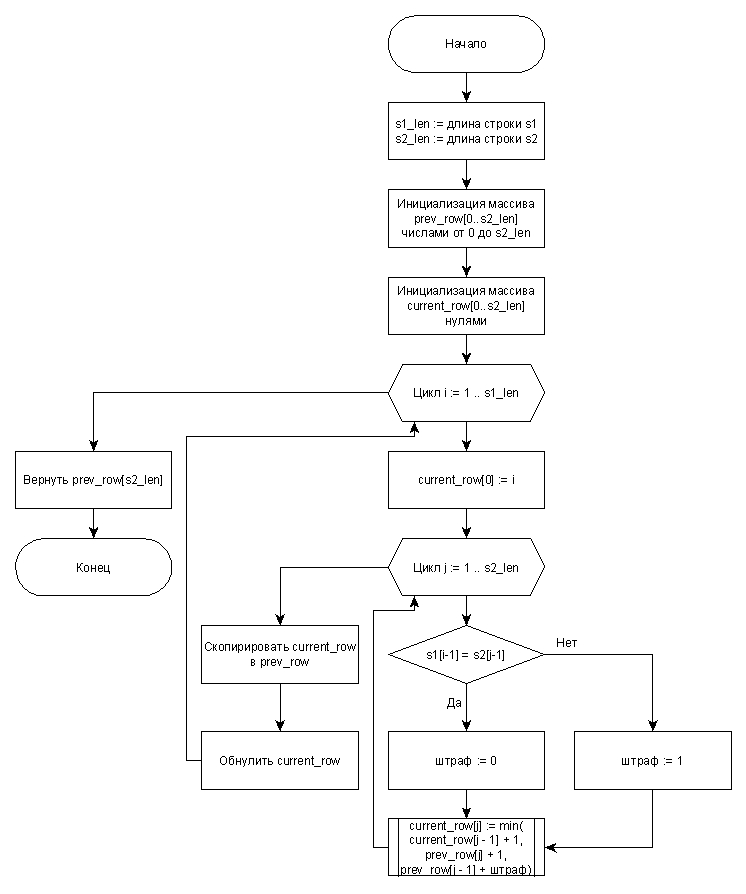
\includegraphics[scale=0.5]{leven}
		\caption{Алгоритм Левенштейна}
		\label{fig:leven}
	\end{figure}

	\begin{figure}[ht!]
		\centering
		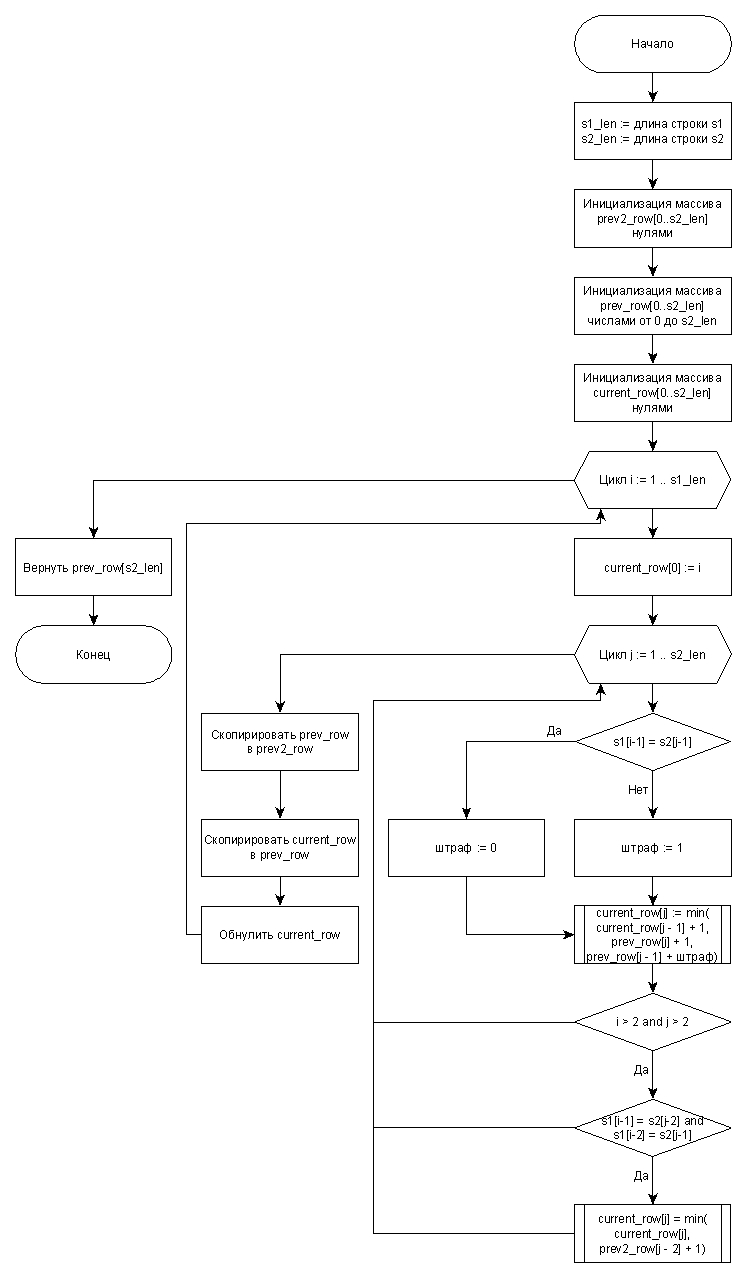
\includegraphics[scale=0.5]{damleven}
		\caption{Матричный алгоритм Дамерау-Левенштейна}
		\label{fig:damleven}
	\end{figure}

	\begin{figure}
		\centering
		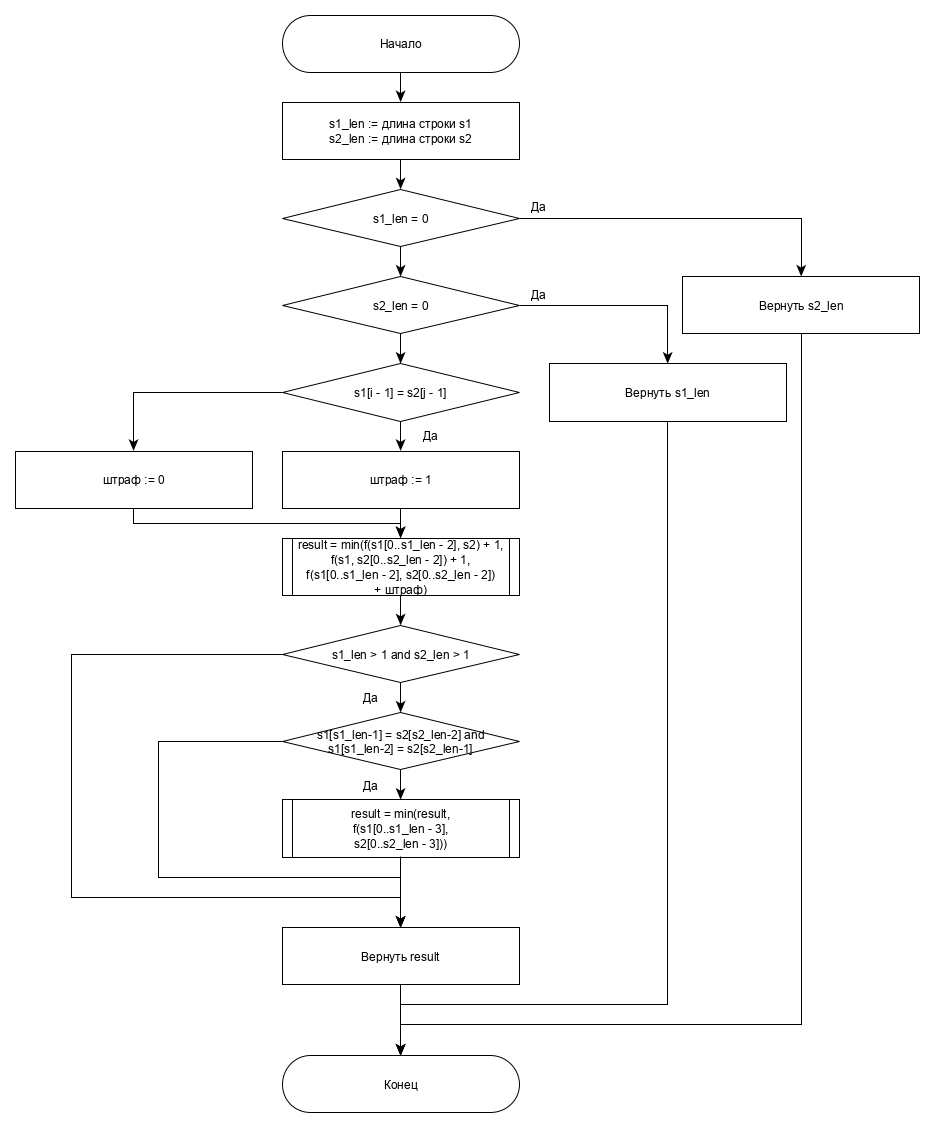
\includegraphics[scale=0.5]{damleven_r}
		\caption{Рекурсивный алгоритм Дамерау-Левенштейна}
		\label{fig:damlevenr}
	\end{figure}

	\newpage
	
	\chapter{Технологическая часть}
	\section{Требования к программному обеспечению}
	На вход подаются две строки, символы которой входят в таблицу Юникода (UTF-16). На выход программа выдаёт три числовых значения, которые являются результатами вычисления расстояний тремя методам: матричными алгоритмоми Левенштейна и Дамерау-Левенштейна и рекурсивным алгоритмом Дамерау-Левенштейна. В качестве результата для матричных алгоритмов также выводится матрица вычислений.
	\section{Средства реализации}
	Для реализации программы был использован язык Python ~\cite{Python}, так как данный язык позволяет проще работать с символьными строками: для того чтобы отбросить последние символы строки (что требуется при реализации рекурсивного алгоритма) имеется возможность использовать встроенные методы - срезы. Для написания функции замера времени был использован язык C ~\cite{C}, так как данный язык имеет в составе стандартной библиотеки встроенную функцию замера процессорного времени в тиках.
	\section{Листинг кода}
	\begin{lstlisting}[label=some-code,caption=Расстояние Левенштейна (матрично)]
	def str_distance(s1, s2, to_print=False):
	    s1_len = len(s1)
	    s2_len = len(s2)
	
	    # initialization of first two rows
	    prev_row = [i for i in range(s2_len + 1)]   # first row - [0, 1, ..., n]
	    current_row = [0] * (s2_len + 1)
	
	    if to_print:
	        print(prev_row)
	
	    for i in range(1, s1_len + 1):          # row loop
	        # current row fill
	        current_row[0] = i
	        for j in range(1, s2_len + 1):                  # column loop
	            match_fault = int(s1[i - 1] != s2[j - 1])            # symbol match
	            current_row[j] = min(current_row[j - 1] + 1,         # horizontal
	                                 prev_row[j] + 1,                # vertical
	                                 prev_row[j - 1] + match_fault)  # diagonal
	
	        if to_print:
	            print(current_row)
	
	        # row switching
	        prev_row = current_row
	        current_row = [0] * (s2_len + 1)
	
	    return prev_row[-1]     # value in bottom right corner of table
	\end{lstlisting}

	\begin{lstlisting}[label=some-code,caption=Расстояние Дамерау-Левенштейна (матрично)]
	def str_distance(s1, s2, to_print=False):
    s1_len = len(s1)
    s2_len = len(s2)

    # initialization of first two rows
    prev2_row = [0] * (s2_len + 1)
    prev_row = [i for i in range(s2_len + 1)]
    current_row = [0] * (s2_len + 1)

    if to_print:
        print(prev_row)

    for i in range(1, s1_len + 1):          # row loop
        # current row fill
        current_row[0] = i
        for j in range(1, s2_len + 1):                  # column loop
            match_fault = int(s1[i - 1] != s2[j - 1])      # if symbol matches
            current_row[j] = min(current_row[j - 1] + 1,         # horizontal
                                 prev_row[j] + 1,                # vertical
                                 prev_row[j - 1] + match_fault)  # diagonal

            # transposition check
            if i > 2 and j > 2:
                if s1[i - 1] == s2[j - 2] and s1[i - 2] == s2[j - 1]:
                    current_row[j] = min(current_row[j],
                                         prev2_row[j - 2] + 1)

        if to_print:
            print(current_row)

        # row switching
        prev2_row = prev_row
        prev_row = current_row
        current_row = [0] * (s2_len + 1)

    return prev_row[-1]         # value in bottom right corner of table
	\end{lstlisting}

	\begin{lstlisting}[label=some-code,caption=Расстояние Дамерау-Левенштейна (рекурсивно)]
		def str_distance(s1, s2):
	    s1_len = len(s1)
	    s2_len = len(s2)
	
	    if s1_len == 0:
	        return s2_len
	    if s2_len == 0:
	        return s1_len
	
	    match_fault = int(s1[-1] != s2[-1])
	
	    result = min(str_distance(s1[:-1], s2) + 1,
	                 str_distance(s1, s2[:-1]) + 1,
	                 str_distance(s1[:-1], s2[:-1]) + match_fault)
	
	    if s1_len > 1 and s2_len > 1:
	        if s1[-1] == s2[-2] and s1[-2] == s2[-1]:
	            result = min(result, str_distance(s1[:-2], s2[:-2]) + 1)
	
	    return result
	\end{lstlisting}
	
	\lstset{ %
	language=C++,                 % выбор языка для подсветки (здесь это С)
	basicstyle=\small\sffamily, % размер и начертание шрифта для подсветки кода
	numbers=left,               % где поставить нумерацию строк (слева\справа)
	numberstyle=\tiny,           % размер шрифта для номеров строк
	stepnumber=1,                   % размер шага между двумя номерами строк
	numbersep=-5pt,                % как далеко отстоят номера строк от         подсвечиваемого кода
	backgroundcolor=\color{white}, % цвет фона подсветки - используем         \usepackage{color}
	showspaces=false,            % показывать или нет пробелы специальными     отступами
	showstringspaces=false,      % показывать или нет пробелы в строках
	showtabs=false,             % показывать или нет табуляцию в строках
	frame=single,              % рисовать рамку вокруг кода
	tabsize=2,                 % размер табуляции по умолчанию равен 2 пробелам
	captionpos=t,              % позиция заголовка вверху [t] или внизу [b] 
	breaklines=true,           % автоматически переносить строки (да\нет)
	breakatwhitespace=false, % переносить строки только если есть пробел
	escapeinside={\%*}{*)},   % если нужно добавить комментарии в коде
	keywordstyle=\color{blue}\ttfamily,
	stringstyle=\color{red}\ttfamily,
	commentstyle=\color{green}\ttfamily,
	morecomment=[l][\color{magenta}]{\#},
	columns=fullflexible }
	\begin{lstlisting}[label=time,caption=Функция замера времени]
	unsigned long long tick(void)
	{
		unsigned long long d;
		__asm__ __volatile__("rdtsc" : "=A"(d));
		return d;
	}
	\end{lstlisting}

	\newpage

	\section{Тесты}
	Для проверки корректности работы были подготовлены следующие функциональные тесты:\\
	\begin{table}[ht!]
		\begin{tabular}{|c|c|c|c|}
		\hline
		\bf{Строка 1} & \bf{Строка 2} & \bf{Ожидание} & \bf{Результат}\\\hline
		<пустая> & <пустая> & 0 0 0 & 0 0 0\\\hline
		<пустая> & а & 1 1 1 & 1 1 1\\\hline
		а & <пустая> & 1 1 1 & 1 1 1\\\hline
		а & а & 0 0 0 & 0 0 0\\\hline
		а & б & 1 1 1 & 1 1 1\\\hline
		азы & базы & 1 1 1 & 1 1 1\\\hline
		компютер & компьютер & 1 1 1 & 1 1 1\\\hline
		данны & данные & 1 1 1 & 1 1 1\\\hline
		email.ru & mail.ru & 1 1 1 & 1 1 1\\\hline
		programmmer & programmer & 1 1 1 & 1 1 1\\\hline
		mail.rus & mail.ru & 1 1 1 & 1 1 1\\\hline
		ашибка & ошибка & 1 1 1 & 1 1 1\\\hline
		алгоритм & алгорифм & 1 1 1 & 1 1 1\\\hline
		копия & копии & 1 1 1 & 1 1 1\\\hline
		укрсовой & курсовой & 2 1 1 & 2 1 1\\\hline
		аглоритм & алгоритм & 2 1 1 & 2 1 1\\\hline
		унивре & универ & 2 1 1 & 2 1 1\\\hline
		курс & курсовой & 4 4 4 & 4 4 4\\\hline
		курсовой & курс & 4 4 4 & 4 4 4\\\hline
		курсовой & курсовик & 2 2 2 & 2 2 2\\\hline
		код & закодировать & 9 9 9 & 9 9 9\\\hline
		закодировать & код & 9 9 9 & 9 9 9\\\hline
		ccoders & recoding & 5 5 5 & 5 5 5\\\hline
		header & subheader & 3 3 3 & 3 3 3\\\hline
		subheader & header & 3 3 3 & 3 3 3\\\hline
		subheader & overheader & 4 4 4 & 4 4 4\\\hline
		\end{tabular}
		\caption{Функциональные тесты}
	\end{table}

	\chapter{Экспериментальная часть}
	\section{Примеры работы}
	\begin{figure}[ht!]
		\centering
		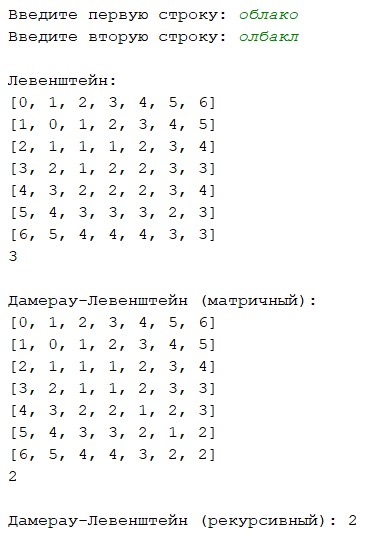
\includegraphics[width=0.4\linewidth]{example}
		\caption{Пример работы программы}
		\label{fig:example}
	\end{figure}
	
	\section{Сравнение работы алгоритмов Левенштейна и Дамерау-Левенштейна}
	Для сравнения времени работы алгоритмов Левенштейна и Дамерау-Левенштейна были использованы строки длиной от 1 до 7 с шагом 1. Эксперимент для более точного результата повторялся 100 раз. Итоговый результат рассчитывался как средний из полученных результатов.\\
	\pgfplotstabletypeset[
	col sep=semicolon,
	string type,
	columns/Length/.style={column name=Длина слова, column type={|c}},
	columns/Leven/.style={column name=Левенштейн, column type={|c}},
	columns/DamerauM/.style={column name=Дамерау-Левенштейн (матричный), column type={|c}},
	columns/DamerauR/.style={column name=Дамерау-Левенштейн (рекурсивный), column type={|c|}},
	every head row/.style={before row=\hline,after row=\hline},
	every last row/.style={after row=\hline},
	]{TimeResults.csv}
	
	\begin{tikzpicture}
	\begin{axis}
		[%title = Сравнение времени работы алгоритмов Левенштейна и Дамерау-Левенштейна,
		table/col sep = semicolon,
		xlabel={Количество символов},
		ylabel={Время в тиках},
		ymin = 0,
		legend pos=outer north east,
		ymajorgrids=true,
		grid style=dashed]
		\addplot[color=red, mark=*] table[x={Length}, y={Leven}] {TimeResults.csv};
		\addplot[color=blue, mark=*] table[x={Length}, y={DamerauM}] {TimeResults.csv};
		\legend{Алгоритм Левенштейна, Алгоритм Дамерау-Левенштейна}
	\end{axis}
	\end{tikzpicture}
	\vspace{1cm}
	
	Алгоритм Левенштейна выигрывает по времени в среднем не более, чем на 10 процентов. При этом алгоритм Дамерау-Левенштейна даёт наилучший результат. Исходя из этого, можно сделать вывод о том, что из матричных методов эффективнее использовать алгоритм Дамерау-Левенштейна.
   
	\section{Сравнение работы реализаций алгоритма Дамерау-Левенштейна}
	Для сравнения времени работы матричной и рекурсивной реализаций алгоритма Дамерау-Левенштейна были использованы строки длиной от 1 до 7 с шагом 1. Эксперимент для более точного результата повторялся 100 раз. Итоговый результат рассчитывался как средний из полученных результатов.\\
	\begin{tikzpicture}
	\begin{axis}
		[%title = Сравнение времени работы матричной и рекурсивной реализации алгоритма Левенштейна,
		table/col sep = semicolon,
		xlabel={Количество символов},
		ylabel={Время в тиках},
		ymin = 0,
		legend pos=outer north east,
		ymajorgrids=true,
		grid style=dashed]
		\addplot[color=red, mark=*] table[x={Length}, y={DamerauM}] {TimeResults.csv};
		\addplot[color=blue, mark=*] table[x={Length}, y={DamerauR}] {TimeResults.csv};
		\legend{Матричная реализация, Рекурсивная реализация}
	\end{axis}
	\end{tikzpicture}
	\vspace{1cm}
	
 	Время выполнения рекурсивного алгоритма резко возрастает с увеличением длины слов: так при длине слова 5 рекурсивный алгоритм выполняется в 50 раз дольше, чем матричный. Рекурсивный алгоритм выигрывает по времени только при длине слов, равной 1 (на 37 процентов). Можно сделать вывод о том, что матричный алгоритма значительно эффективнее рекурсивного.

	\chapter*{Заключение}
	\addcontentsline{toc}{chapter}{Заключение}
	Алгоритмы нахождения расстояния Левенштейна и Дамерау-Левенштейна между строками были изучены и реализованы: были реализованы три варианта алгоритма для получения навыка динамического программирования.\\
	Были исследованы затраты данных вариантов реализации по времени и памяти. Экспериментально было подтверждено, что рекурсивный вариант реализации алгоритма значительно проигрывает матричным вариантам при росте длины входных строк по обоим показателям.

	\newpage
	
	\begin{thebibliography}{}
	\bibitem{leven} Двоичные коды с исправлением выпадений, вставок и замещений символов. Доклады Академий Наук СССР, 1965. В. И. Левенштейн.
	\bibitem{damerau} A technique for computer detection and correction of spelling errors. Damerau Fred J.
	\bibitem{Python} https://www.python.org/doc/ [Электронный ресурс]
	\bibitem{C} https://creference.com/ [Электронный ресурс]
	\bibitem{recurs} Indexing methods for approximate dictionary searching. Journal of Experimental Algorithmics, 2011. L. M. Boytsov
	\end{thebibliography}
	\addcontentsline{toc}{chapter}{Литература}

\end{document}
